\section{案例研究：RMSNorm}
\label{sec:case2}

在本节中，我们以均方根层归一化（RMSNorm）~\cite{zhang2019rootmeansquarelayer} 为案例研究，展示 \graph 表示和 \sys 超级优化方法的优势。
RMSNorm 是近期大型语言模型中广泛使用的归一化技术~\cite{grattafiori2024llama3herdmodels}。形式上，RMSNorm 接收两个张量 $X$ 和 $G$ 作为输入，并根据均方根对其逐元素乘积进行归一化：
\begin{equation}
    Y_{ij} = \frac{X_{ij}G_j}{\textrm{RMS}(X_i)}, \quad \textrm{RMS}(X_i) = \sqrt{\frac{1}{d}\sum_{j=1}^{d} X_{ij}^2},
\end{equation}
其中 $d$ 是 $X$ 的隐藏维度大小。

\begin{figure}
    \centering
    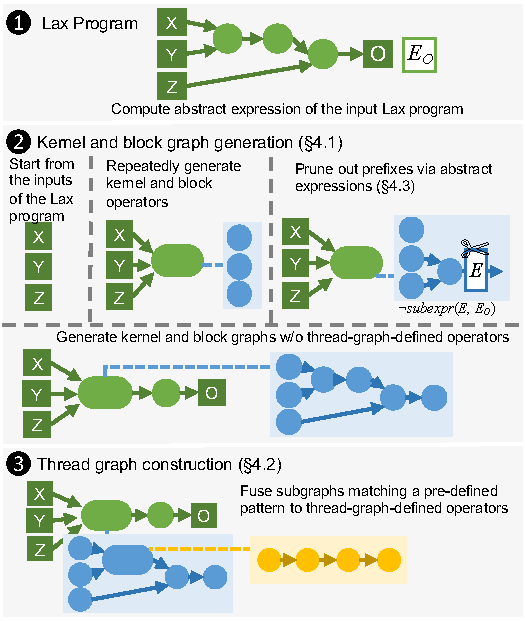
\includegraphics[width=\columnwidth]{figs/generator.pdf}
    \vspace{-1em}
    \caption{\graph 生成器概览。}
    \vspace{\captionvspace}
    \label{fig:generator}
\end{figure}

RMSNorm 之后通常紧跟一个矩阵乘法（MatMul）。\Cref{fig:rms_norm_baseline} 展示了 RMSNorm 后接 MatMul 运算符的计算图，其中 $X$ 是输入张量，$G$ 和 $W$ 表示两个权重张量。
现有机器学习编译器通常为 RMSNorm 和 MatMul 计算分别启动两个独立的核，因为这两个运算在内部都对输入维度进行规约，使得将它们的计算融合到单个核中变得困难。
这种方法需要将中间结果（即 $Y$）存储在设备内存中，因为不同的核无法在共享内存或寄存器文件中共享数据。

\Cref{fig:rms_norm_mlso} 展示了 \sys 为将 RMSNorm 和 MatMul 融合在单个核中自动发现的最优 \graph。该计算被融合在单个图定义核运算符中，以避免将中间结果（即 $Y$）保存到设备内存，并减少核启动开销。

我们重点介绍 \sys 发现的 \graph 与原始 \graph 之间的关键差异。
这些差异涉及发现新的自定义核以及代数变换和调度变换的结合，使得通过单独考虑代数变换和调度变换来发现最终 \graph 是不可行的。
首先，\sys 通过利用矩阵乘法和逐元素除法的交换律（代数变换），对 MatMul 和 RMSNorm 的除法进行重排序。
其次，\sys 并行执行均方根中的累加（即 $A_i = \sum_j X_{ij}^2$）和矩阵乘法中的累加（即 $B_{ik} = \sum_j X_{ij} G_j W_{jk}$）（调度变换），从而避免将累加结果写入设备内存。
接着，\sys 实例化一个线程图，在寄存器文件中执行一系列逐元素运算符，同时将所有中间结果保持在寄存器文件中（调度变换）。
最后，发现的最优 \graph 使用一个新的自定义核来融合 RMSNorm 和 MatMul 的计算，减少设备内存访问和核启动开销。该 \graph 在 NVIDIA A100 和 H100 GPU 上分别比现有系统中的手写核性能提升 $1.5\times$ 和 $1.9\times$。
